%%% Template originaly created by Karol Kozioł (mail@karol-koziol.net) and modified for ShareLaTeX use

\documentclass[a4paper,11pt]{article}

\usepackage[T1]{fontenc}
\usepackage[utf8]{inputenc}
\usepackage{graphicx}
\usepackage{xcolor}

\usepackage{tgtermes}

\usepackage[
pdftitle={CS 663 : Digital Image Processing : Assignment 1}, 
pdfauthor={Kalpesh Krishna, Pranav Sankhe, Mohit Madan},
colorlinks=true,linkcolor=blue,urlcolor=blue,citecolor=blue,bookmarks=true,
bookmarksopenlevel=2]{hyperref}
\usepackage{amsmath,amssymb,amsthm,textcomp}
\usepackage{enumerate}
\usepackage{multicol}
\usepackage{tikz}

\usepackage{geometry}
\geometry{total={210mm,297mm},
left=25mm,right=25mm,%
bindingoffset=0mm, top=20mm,bottom=20mm}


\linespread{1.3}

\newcommand{\linia}{\rule{\linewidth}{0.5pt}}

% custom theorems if needed
\newtheoremstyle{mytheor}
    {1ex}{1ex}{\normalfont}{0pt}{\scshape}{.}{1ex}
    {{\thmname{#1 }}{\thmnumber{#2}}{\thmnote{ (#3)}}}

\theoremstyle{mytheor}
\newtheorem{defi}{Definition}

% my own titles
\makeatletter
\renewcommand{\maketitle}{
\begin{center}
\vspace{2ex}
{\huge \textsc{\@title}}
\vspace{1ex}
\\
\linia\\
\@author \hfill \@date
\vspace{4ex}
\end{center}
}
\makeatother
%%%

% custom footers and headers
\usepackage{fancyhdr,lastpage}
\pagestyle{fancy}
\lhead{}
\chead{}
\rhead{}
\lfoot{Assignment \textnumero{} 5}
\cfoot{}
\rfoot{Page \thepage\ /\ \pageref*{LastPage}}
\renewcommand{\headrulewidth}{0pt}
\renewcommand{\footrulewidth}{0pt}
%

%%%----------%%%----------%%%----------%%%----------%%%

\begin{document}

\title{EE 309 : Microprocessor Project 1 : IITB RISC}

\author{Pranav Sankhe, Sachin Goyal, Srivatsan Shridhar, Tanya Chaudhary}

\date{8/11/2017}

\maketitle


\section{Datapath Design \& Description}

\subsection{Datapath Design}
\begin{figure}[h!]
  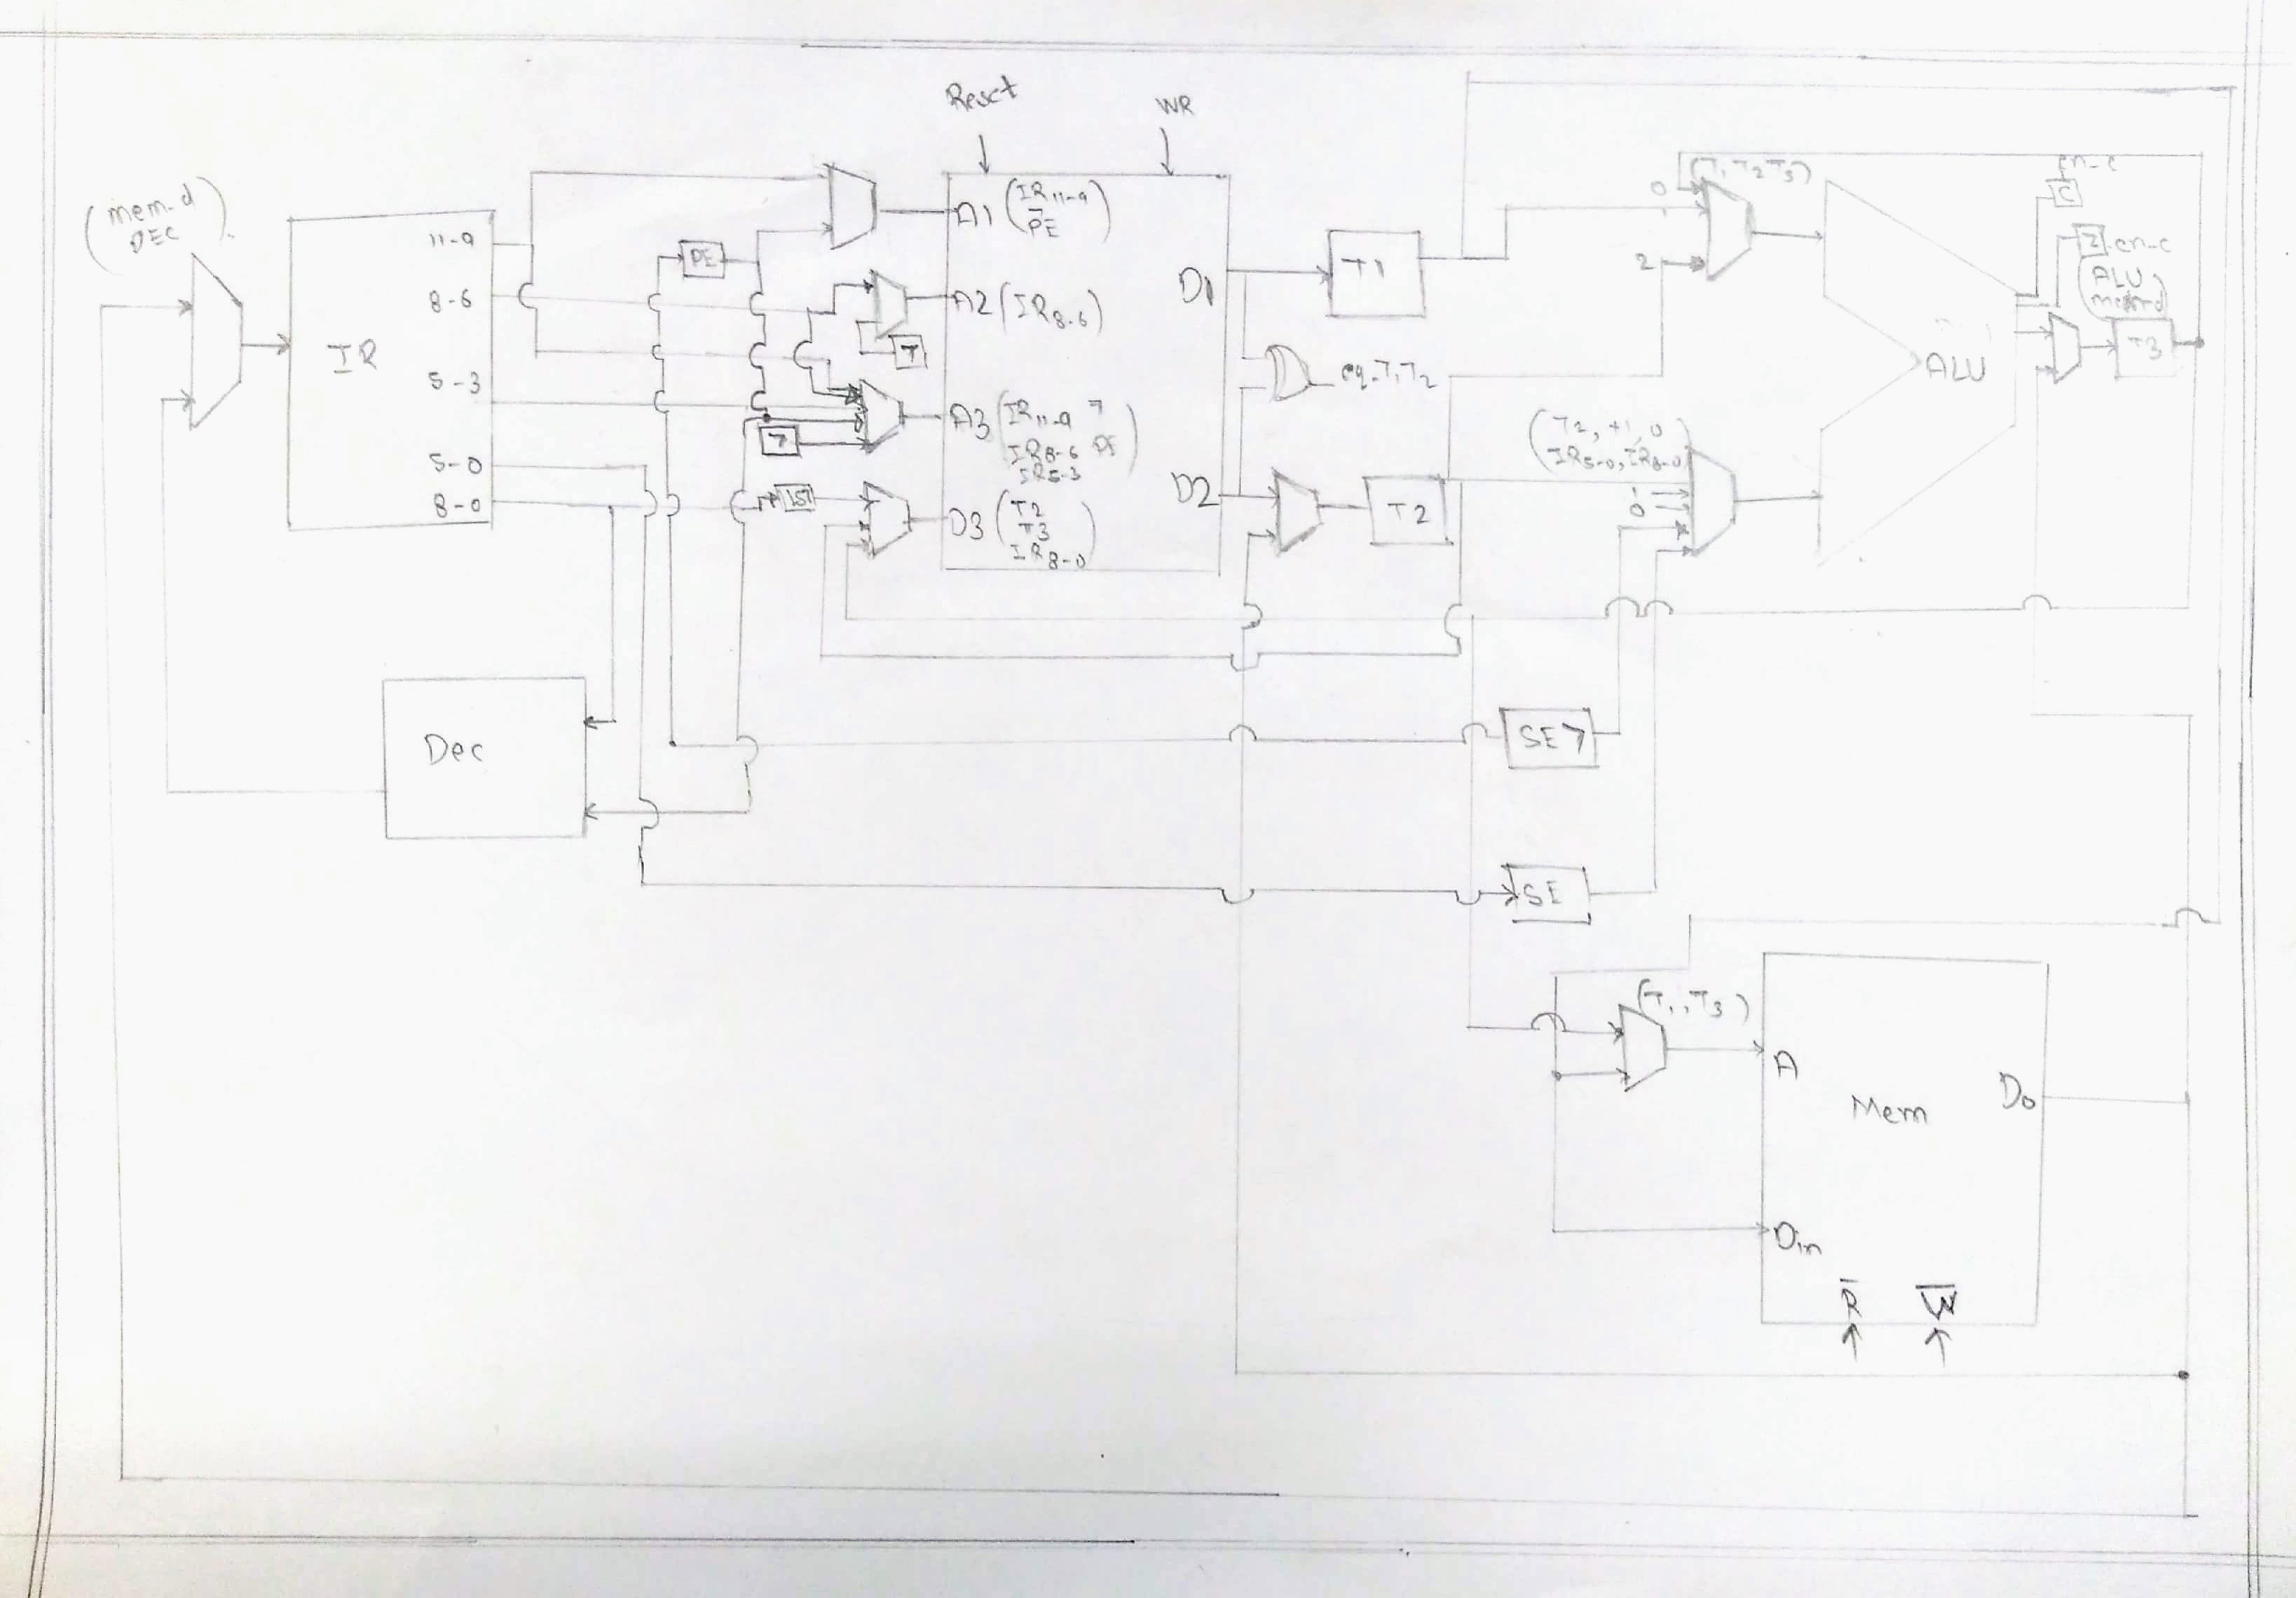
\includegraphics[width=\linewidth]{micro.jpg}
  \label{fig:result1}
\end{figure}

\subsection{Description}

\begin{itemize}
\item \textbf{Memory}\\
We have 16 bit addresses in memory, and each address stores 16 bit data in it. The memory block is controlled by R and W signals.   
\item \textbf{Register File}\\
Register file has 4 inputs A1, A2, A3, D3 and 2 outputs D1 and D2. It is controlled by 2 signals Reset and WR. 
\item \textbf{ALU}\\ 
Our ALU supports AND and NAND instructions. It sets the Z(zero) and C(carry) flag after instruction.  

\end{itemize}



\section{Flowchart Design}

\begin{figure}[h!]
  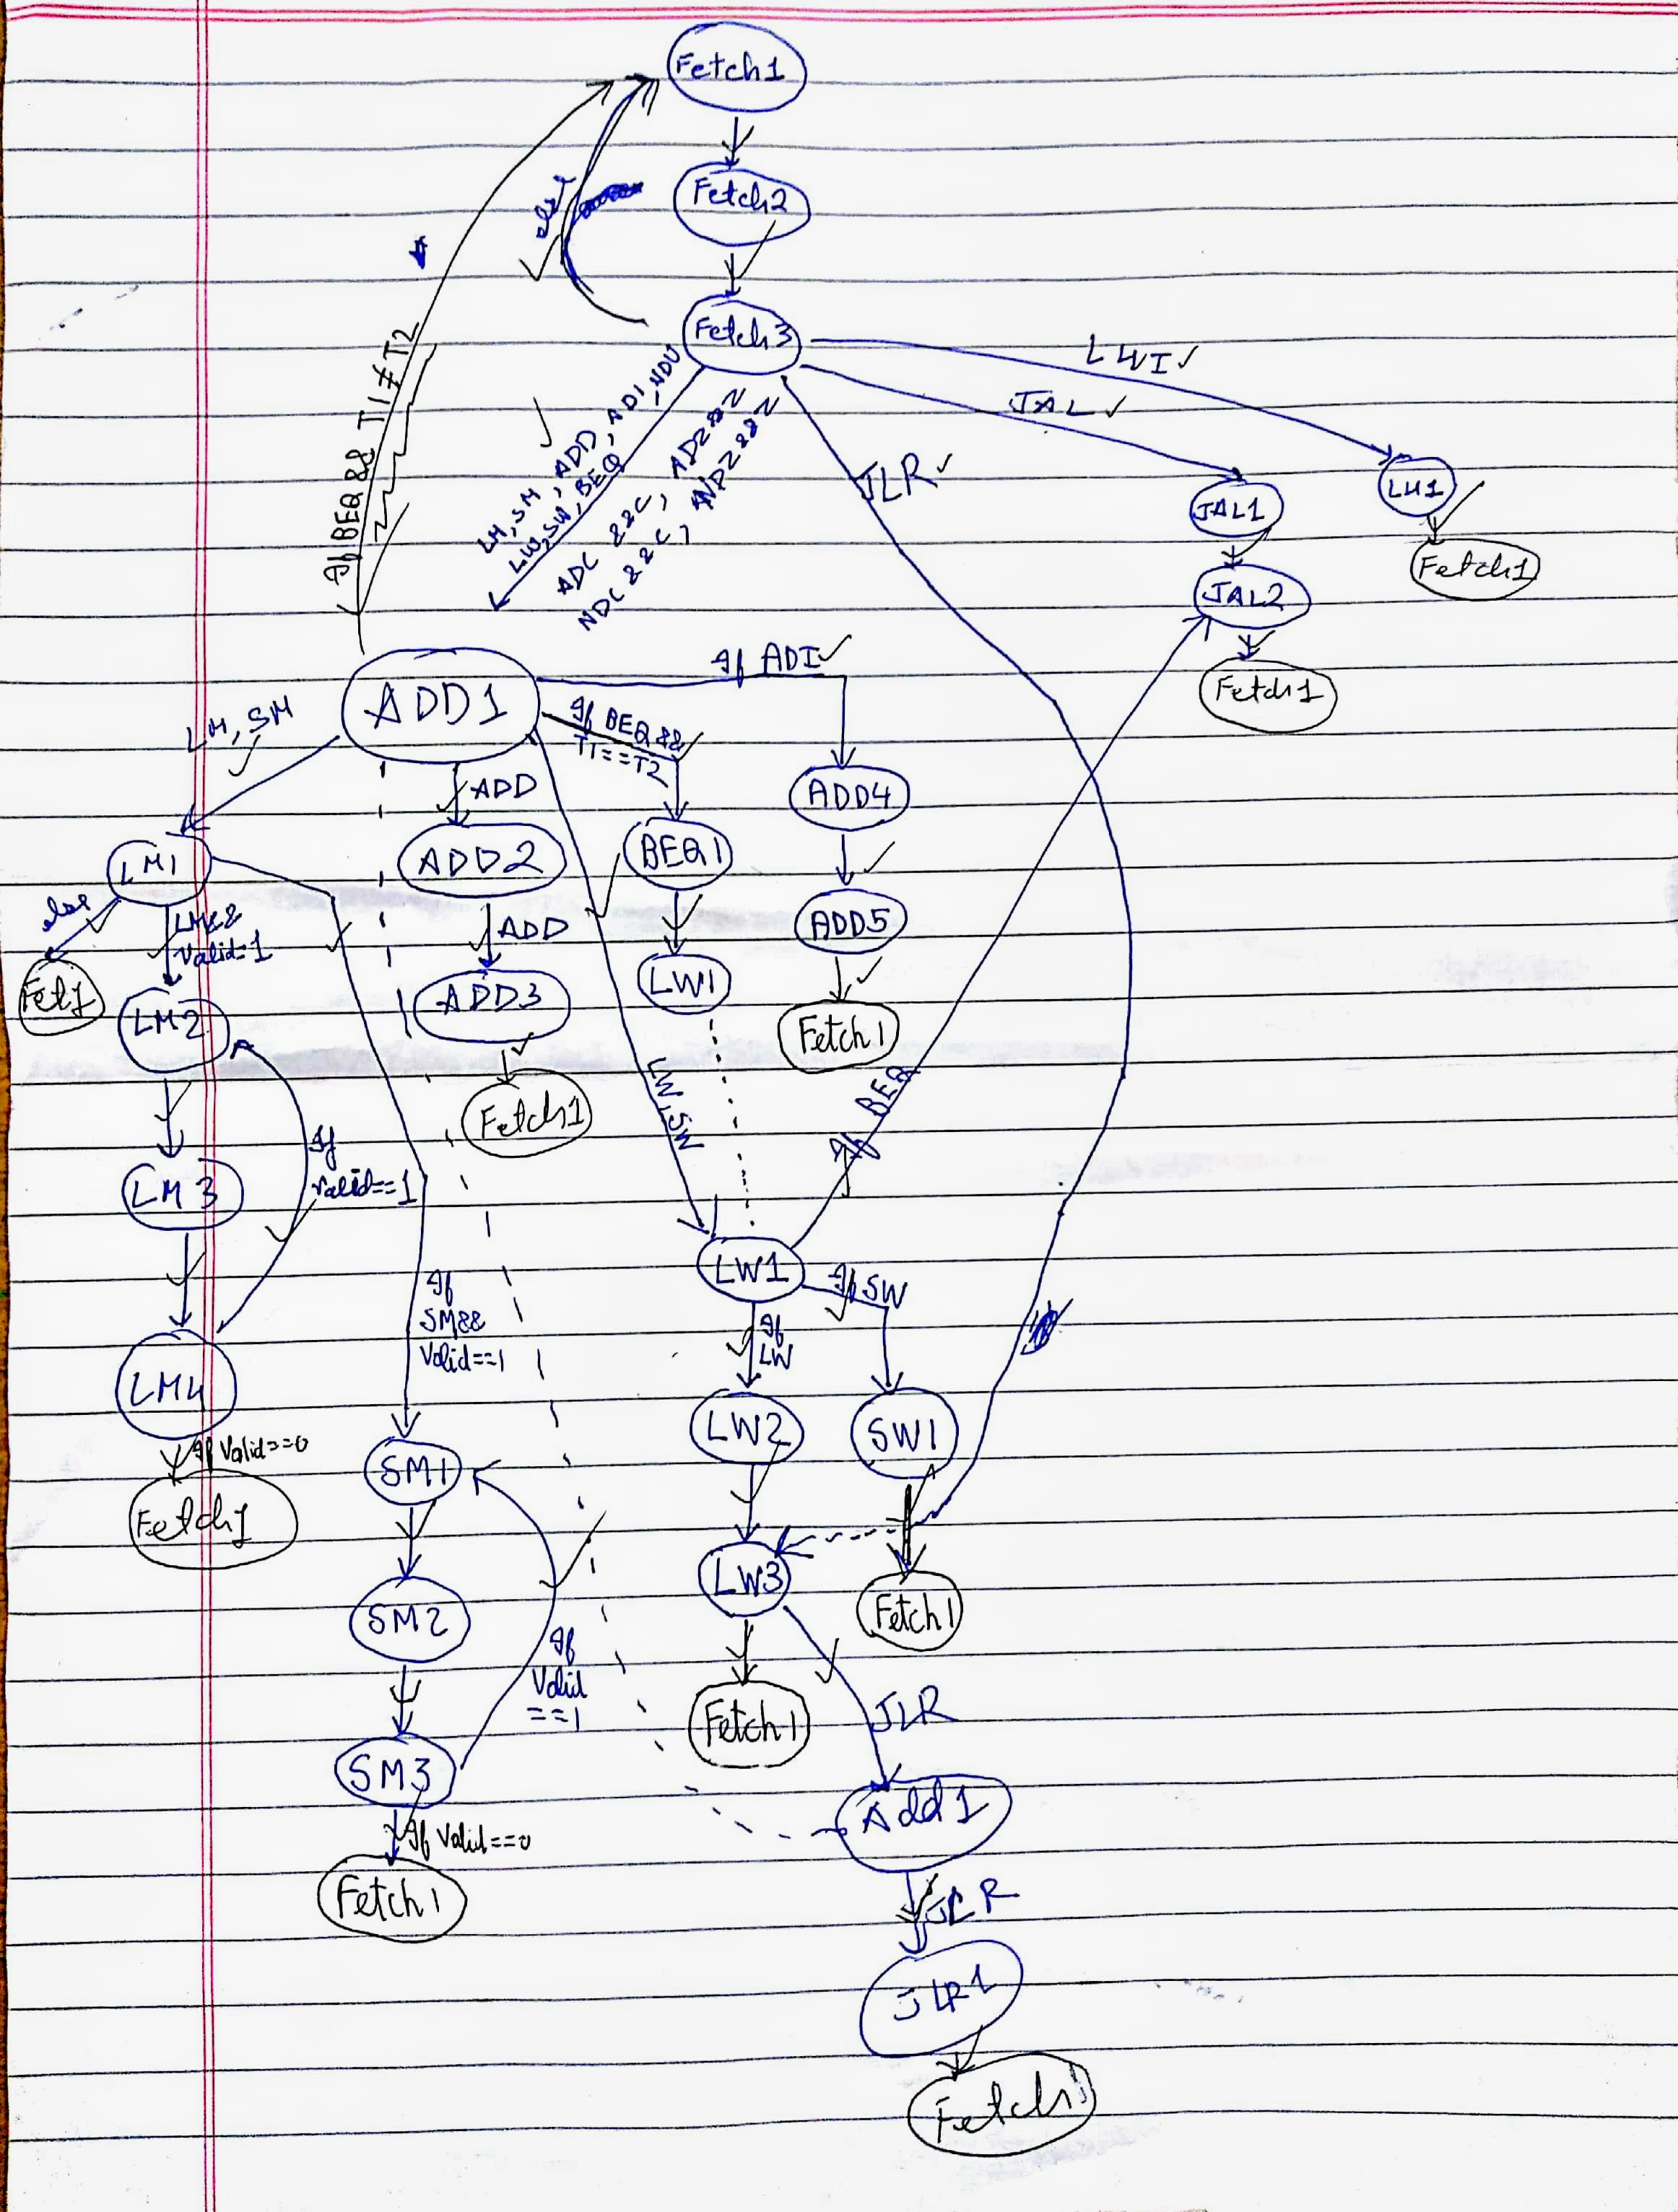
\includegraphics[width=\linewidth]{flow_chart.jpg}
  \label{fig:result1}
\end{figure}



\section{Test Cases}

\end{document}
